

%%-----------------------------------------------------
%%-----------------------------------------------------
\section{Navegando sin bloqueos IP}


%-----------------------    ---------------------------------

\begin{frame}
\frametitle{Problema}

\begin{itemize}
   \item Muchas veces, especialmente con contenidos audiovisuales, existen
   restricciones según el país de acceso
   \item Los servidores de contenido toman como punto de partida la asignación
   de la IP de nuestra máquina para bloquearnos
\end{itemize}

\end{frame}

%-----------------------    ---------------------------------

\begin{frame}
\frametitle{Solución}

\begin{itemize}
   \item Uso de \emph{virtual private networks}
   \item Hay muchos servicios que ofrecen este servicio pagando una cuota mensual
   \begin{itemize}
     \item \url{https://vpncreative.net/vpn-providers/}
   \end{itemize}
   \item Tres servicios:
   \begin{itemize}
     \item Proxy
     \item Privacidad (*)
     \item Seguridad
   \end{itemize}
\end{itemize}

\end{frame}



%-----------------------    ---------------------------------

\begin{frame}
\frametitle{VPN para descargas masivas}

\begin{center}
  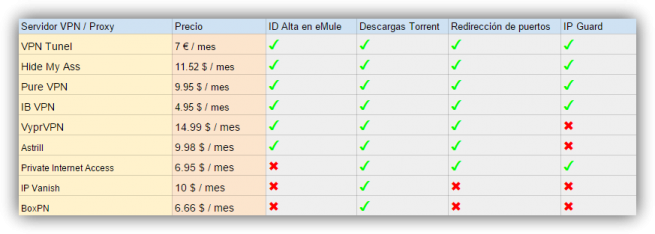
\includegraphics[width=11cm]{figs/vpn-proxy.png}
\end{center}


\begin{flushright}
{\tiny
Source: ADSL Zone (enero 2015)
}
\end{flushright}

\end{frame}





